\chapter{Design}\label{chap:design}

In diesem Kapitel findet sich der Entwurf der entwickelten Komponenten. Dabei geht es vor allem um die Komposition und geplanten Aufbau der Elemente Emulator, (Dis-)Assembler und Frontend. Sie bilden die zentralen Bestandteile der vorliegenden Arbeit und dementsprechend wird ihr Aufbau mit geplanten Schnittstellen vorgestellt. Während der Fokus auf der logischen Zusammensetzung und ihrer geplanten Umsetzung liegt, werden Codebeispiele herangezogen um bestimmte Grundlagen noch vor der Implementierung in Kapitel \ref{chap:impl} zu verdeutlichen.

\section{Emulator}

Der Emulator umfasst alles, was zur Simulation der Intel 8080 \ac{CPU} beiträgt. Dabei handelt es sich hauptsächlich um das Ausführen von Instruktionen, das Interrupt-Handling sowie die Anbindung von Ein- und Ausgabegeräten.

\subsection{Zentrale Struktur}

\begin{listing}[ht]
\begin{minted}{rust}
    struct Emulator {
        pc: u16,
        sp: u16,
        ram: RAM,
        reg: RegisterArray,
        input_devices: [InputDevice; 256],
        output_devices: [OutputDevice; 256],
        running: bool,
        interrupts_enabled: bool
    }
\end{minted}
\centering
\caption{Zentrale Emulator Struktur}
\label{lst:wtf}
\end{listing}

Den Kern des Emulators bildet eine Struktur, welche zuständig für die Ausführung der Maschinencode-Programme ist. Sie gruppiert alle notwendigen Komponenten eines Intel 8080 Systems. Der Aufbau der Struktur ist in \cref{lst:wtf} illustriert.

Diese Komponenten wurden in \cref{chap:prereqs} bereits erklärt: \rust{pc} und \rust{sp} sind zwei 16-Bit-Zahlen, die den \ac{PC} und den \ac{SP} repräsentieren. \rust{ram} ist der Arbeitsspeicher und \rust{reg} simuliert die Register (inklusive Flags und Akkumulator).
Die Ports für I/O-Geräte werden durch zwei Arrays mit jeweils 256 Elementen repräsentiert.
Darauf folgen zwei Boolean, einer sagt aus, ob der Emulator am Laufen ist und der andere gibt an, ob Interrupts erlaubt sind.


\subsection{Modularität}

Der Intel 8080 ist lediglich die \ac{CPU} --- \ac{RAM} und I/O-Geräte arbeiten prinzipiell unabhängig. Diese müssen zwar eine entsprechende Schnittstelle bereitstellen um angeschlossen werden zu können, aber können beliebig implementiert sein. Die Implementierung ermöglicht es verschiedene Implementierungen für \ac{RAM} und Input/Output-Devices zu haben. Bei diesen Typen handelt es sich um die in Kapitel \ref{chap:traits} vorgestellten Traits.

\subsection{Ausführung}

Die Methode \rust{Emulator::execute_next()} führt die Instruktion aus, auf die der \ac{PC} zeigt. Der Opcode wird über ein enormes \rust{match}-Statement auf die entsprechende Funktion delegiert, mittels welcher die Operation ausgeführt wird. Diese Funktionen sind dafür zuständig, den \ac{PC} entsprechend zu erhöhen. Abhängig vom ausgeführten Opcode muss dieser um eins, zwei oder drei erhöht werden.

Der Rückgabetyp der Methode ist \rust{Result<(), &str>}, dadurch können entsprechende Fehlermeldungen nach außen propagiert werden. Dies ist wünschenswert, damit auf dem Frontend entsprechende Fehlermeldungen angezeigt werden können, um dem Benutzer den Entwicklungsprozess zu erleichtern.

\subsubsection{Instruktionen}

Um zu großen Dateien vorzubeugen, sind die Implementierungen der Instruktionen in verschiedene Module aufgeteilt. Sie sind logisch gruppiert in Arithmetik, Kontrollfluss, Logik, Speicherzugriff, Verschiebung und Speziell. Obwohl die Funktionen in unterschiedlichen Dateien/Modulen deklariert sind, sind sie Methoden des \rust{Emulator}-Structs. Die verschiedenen Funktionen werden dann im Code von \rust{Emulator::execute_next()} aufgerufen. Auch diese Funktionen geben häufig \rust{Result}s zurück, sofern die Ausführung in einem Fehler resultieren kann.

\subsection{Interrupts}

Über den \rust{interrupts_enabled}-Boolean wird geregelt, ob es erlaubt ist, Interrupts an den Emulator zu senden. Die Folgende Methode der zentralen Struktur wird verwendet, um Interrupts auszulösen:

\begin{minted}{rust}
    pub fn interrupt(&mut self, opcode: u8) -> EResult<usize> {
        if self.interrupts_enabled {
            self.interrupts_enabled = false;
            return self.execute_instruction(opcode);
        }
        Err("Interrupts disabled")
    }
\end{minted}

Wenn Interrupts erlaubt sind, wird der übergebene Opcode ausgeführt und der Boolean invertiert, andernfalls wird eine Fehlermeldung zurückgegeben. \rust{interrupts_enabled} ist initial \rust{false} und muss durch die entsprechende Instruktion (\asm{EI}) gesetzt werden.
Prinzipiell kann jede 1 Byte große Instruktion (parameterlose Instruktion) als Interrupt ausgeführt werden, meistens wird jedoch eine der \asm{RST}-Instruktionen ausgeführt. Diese sind \asm{CALL}-Instruktionen, die zu einer fixen Speicheradresse springen. An diesen fixen Adressen kann der Programmierer die entsprechenden Interrupt-Routinen platzieren.

\section{Assembler}

Für den Emulator und andere Konsumenten des Assemblers soll dieser eine einzelne, geschlossene Schnittstelle sein. Dabei vereint er unterschiedliche Funktionalitäten, die in drei Modulen realisiert werden. Es findet eine funktionelle Aufteilung in die folgenden Dateien statt:

\begin{itemize}
	\item Der eigentliche Assembler zum Übersetzen von Assemblycode und als öffentliche Schnittstelle
	\item Ein Präprozessor zur Behandlung von Pseudo-Instruktionen
	\item Ein Parser zur Auswertung numerischer Werte in unterschiedlichen Formaten
\end{itemize}

Um seine Funktionalität vollständig zu erfüllen soll der Assembler lediglich den vom Nutzer geschriebenen Code benötigen. Darauf aufbauend delegiert er dessen Verarbeitung intern mit Methodenaufrufen des Präprozessors.

Der Präprozessor ist eine \glqq Pure Fabrication\grqq{} für den Assembler. Zwar gibt es in Rust keine Klassen, die eigentlich solche reinen Erfindungen sind, in diesem Fall wird das Konzept von einer Datei umgesetzt. Dabei beinhaltet diese diverse Methoden zum Verarbeiten von Pseudo-Instruktionen, wie sie in Kapitel \ref{chap:pseudo-instructions} erläutert sind. Einzeln angewandt, sind die Methoden nur bedingt zu gebrauchen, da sie auf unterschiedlich weit verarbeitetem Code basieren. Deshalb übernimmt der Präprozessor die komplette Vorverarbeitung und bietet dafür die Methode \rust{get_preprocessed_code()} nach außen hin an. Auf dem an dieser Stelle überlieferten Quellcode basierend erstellt die Methode einen Vektor von Instruktionen, die der Assembler in den entsprechenden Bytecode umwandeln kann.

Zusätzlich zur Verarbeitung von Pseudo-Befehlen, soll der Präprozessor das Erstellen einer Map ermöglichen, die einen Zusammenhang zwischen den erzeugten Bytes und den Zeilen, in denen sich der entsprechende Befehl befindet, herstellen. Für diese Funktion bildet der Assembler entsprechend der Idee, die einzige Schnittstelle zu sein, einen Adapter für die Map zum Frontend, wodurch die interne Repräsentation und Implementierung unabhängig von Anforderungen bezüglich des Formats im Frontend wird.

Gemäß der Spezifikation erlaubt der Intel 8080 die Definition numerischer Werte in verschiedensten Formaten, unter anderem als mathematische Ausdrücke oder auch in Binärdarstellung. Um eine einheitliche Darstellung innerhalb von Rust zu gewährleisten und das Auslesen entsprechender Werte zu zentralisieren, nutzen sowohl Assembler als auch Präprozessor einen Parser. Ähnlich der zweiten Komponente handelt es sich hier um eine Pure Fabrication. Der entwickelte Parser nimmt einen mathematischen Ausdruck als String entgegen und erzeugt davon ausgehend eine Menge Token, die stückweise abgearbeitet wird.

\section{Disassembler}

Ein Disassembler übersetzt Maschinencode zurück nach Assembly. Damit kann er zum Beispiel verwendet werden, um fremde Programme verständlich zu machen.
Die Funktionsweise des Disassemblers ist sehr simpel: Die Eingabe wird Byte für Byte durchlaufen, durch ein großes Match-Statement wird der Opcode unterschieden und entsprechend des Opcodes werden 0, 1 oder 2 Bytes an Parametern gelesen. Der Opcode und die Parameter werden dann benutzt, um die entsprechende Assembly-Instruktion als String zu erzeugen. Folgende Methode zeigt einen Ausschnitt aus dem Hauptelement des Disassemblers:

\begin{minted}{rust}
fn decode_next(&mut self) -> Result<String, &'static str> {
    // Get next Opcode
    let instr = self.read_byte();
    match instr {
        0x00 => Ok(String::from("NOP")),
        0x01 => Ok(format!(
            "LXI B,{}",
            Disassembler::fmt_hex::<u16>(self.read_addr())
        )),
        // ...
}
\end{minted}

Der Disassembler liefert einen Iterator über \rust{Result<String, &'static str>}, wobei die Results die einzelnen Zeilen des Assembly Programmes enthalten. Der Iterator läuft bis die Eingabe vollständig abgearbeitet ist.

\section{Frontend}

Die Webanwendung, mit der Nutzer den Emulator schließlich nutzen können, stellt zwei wesentliche Funktionalitäten zur Verfügung, die nachfolgend vorgestellt werden.

\subsection{Code Editor}

Mit einem eingebauten Code Editor können Nutzer direkt in der Webapplikation eigene Assembly-Programme schreiben und direkt ausführen, ohne beispielsweise vorher selbst den Code zu assemblen und dann manuell in den Emulator zu laden zu müssen.

Für den Code-Editor wird eine quelloffene Bibliothek von Microsoft genutzt, der sogenannte \textit{Monaco Editor}. Monaco ist ein browser-basierter Editor, der praktische Funktionalitäten zur Verfügung stellt, wie zum Beispiel Autovervollständigung oder Syntax-Highlighting. Die Bibliothek wird unter anderem auch in dem weit verbreiteten und ebenfalls quelloffenen Code-Editor \textit{Visual Studio Code} genutzt.

\begin{figure}
    \caption{Code-Editor der Webanwendung}
    \centering
    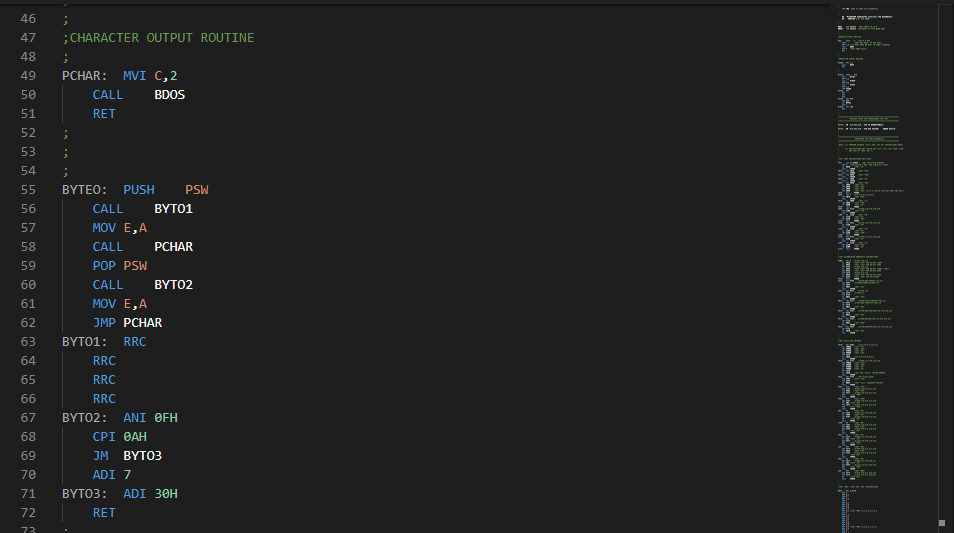
\includegraphics[width=1.0\textwidth]{Bilder/CodeEditor.png}
    \label{fig:codeeditor}
\end{figure}

In Abbildung \ref{fig:codeeditor} sieht man den Code-Editor in Aktion. Die einzelnen Bestandteile des Assembly-Codes, die Labels, die Instruktionen und die Argumente, sowie Kommentare sind alle unterschiedlich eingefärbt.

\begin{figure}
    \caption{Autovervollständigung für Instruktionen}
    \centering
    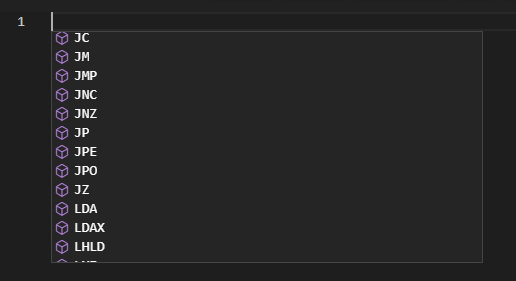
\includegraphics[width=0.6\textwidth]{Bilder/Completion1.png}
    \label{fig:completion1}
\end{figure}

In Abbildung \ref{fig:completion1} sieht man außerdem, wie die Autovervollständigung des Code-Editors funktioniert. Basierend auf der Eingabe des Nutzers und der Position im Code wird automatisch erkannt, ob eine Instruktion oder ein Argument vorgeschlagen werden soll und welche in Frage kommen.

\subsection{Emulator-Zustand}

Hat der Nutzer nun ein Assembly-Programm mithilfe des Code-Editors erstellt, kann er es ausführen. Hierfür wird der in Rust entwickelte Emulator genutzt, der mithilfe der \ac{WASM}-Schnittstelle in die Webapplikation eingebunden wird. Die Interaktion mit dem Emulator erfolgt mithilfe verschiedener Bedienelemente in einer Aktionsleiste am oberen Rand der Anwendung (siehe Abbildung \ref{fig:actionbar}).

\begin{figure}[h]
    \caption{Aktionsleiste des Emulators}
    \centering
    
\includegraphics[width=0.75\textwidth]{Bilder/Aktionsleiste.png}
    \label{fig:actionbar}
\end{figure}

\begin{figure}
    \caption{\textit{Load}-Dialog}
    \centering
    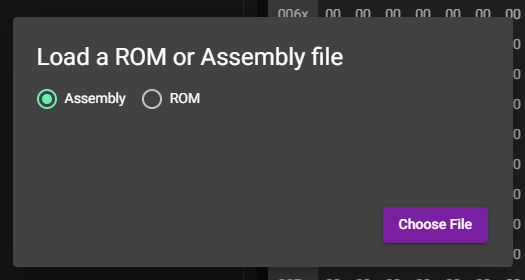
\includegraphics[width=0.75\textwidth]{Bilder/LoadDialog.png}
    \label{fig:loaddialog}
\end{figure}

Die ersten beiden Schaltflächen der Aktionsleiste, \textit{Load} und \textit{Save}, ermöglichen dem Nutzer, Assemblycode aus Dateien von seinem Endgerät zu laden oder sie dort zu speichern. \textit{Load} kann außerdem bereits übersetzten Code direkt in den Speicher des Emulators laden. Die Auswahl erfolgt mithilfe eines eigenen Auswahldialogs, der in Abbildung \ref{fig:loaddialog} zu sehen ist. Wird ein fertiges Programm geladen, kann zusätzlich bestimmt werden, an welcher Stelle es im Arbeitsspeicher platziert werden soll. Dies ist notwendig, da viele Programme beispielsweise erwarten, dass sich der Einstiegspunkt an der Speicheradresse 256 befindet.

Um den Code, den der Nutzer geschrieben hat, nun zu assemblen, muss der Anwender in der Aktionsleiste die Funktion \textit{Assemble} nutzen. Ist der Vorgang erfolgreich, werden die Bytes, die der Assembler erzeugt, in den Hauptspeicher des Emulators geschrieben. Die Emulation kann jetzt mithilfe der grünen Schaltfläche gestartet werden. Da die \ac{CPU} keinen festgelegten Endzustand hat, läuft sie solange weiter, bis der Nutzer die Emulation beendet, was mit dem roten Stopp-Knopf möglich ist.

Um den Ablauf des Codes nachvollziehen zu können, bietet die Applikation die Möglichkeit, jederzeit den internen Status des Prozessors einzusehen. Hierzu existiert auf der rechten Hälfte der Webseite eine Matrix, die den Arbeitsspeicher repräsentiert, sowie eine Anzeige für jedes der Register (siehe Abbildung \ref{fig:cpustate}).

\begin{figure}
    \caption{Anzeigen für den CPU-Status}
    \centering
    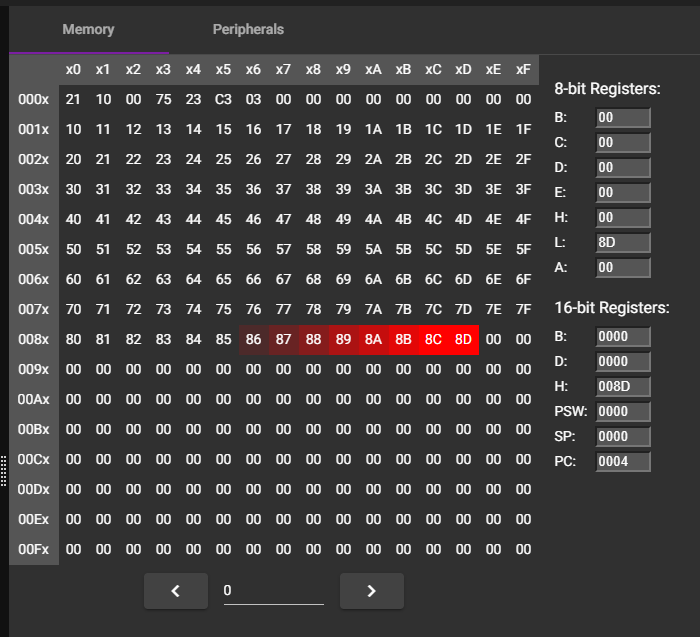
\includegraphics[width=0.75\textwidth]{Bilder/CPUState.png}
    \label{fig:cpustate}
\end{figure}

Die \ac{RAM}-Matrix stellt in jeder Zeile 16 Addressen dar, was die einfache Zuordnung von Zeile zu Spalte mithilfe der letzten Hexadezimalstelle erlaubt. Ändert sich im Arbeitsspeicher durch eine Instruktion des Prozessors ein Wert, wird dieser für eine kurze Zeit rot hinterlegt, um einfacher zu sehen, was sich geändert hat. Da der Speicher in der Regel deutlich größer ist, als die dargestellten 16x16 Bytes, nämlich bis zu 64KB, ist es möglich, den angezeigten Speicherbereich zu verschieben.

Die Registeranzeigen rechts von der \ac{RAM}-Matrix sind in zwei Kategorien gegliedert: Die 8-Bit Register (B, C, D, E, H, L, A) und die 16-Bit Register (BC, DE, HL, PSW, SP, PC).

Die aktuell ausgeführte Instruktion des Prozessors (basierend auf dem \ac{PC}) wird im Code-Editor außerdem rot hinterlegt. Für das Debugging von Programmen gibt es die Möglichkeit, die Ausführung des Emulators mithilfe der gelben Pause-Schaltfläche in der Aktionsleiste zu pausieren. Im pausierten Zustand kann nun jede Instruktion Schritt für Schritt ausgeführt werden.
